% Copyright 2026 Sreeram Anil
% SPDX-License-Identifier: CC-BY-4.0
% =============================================================================
%  Fifth-degree cubature Kalman filter — classical Kalman family
% =============================================================================
\chapter{Fifth-Degree Cubature Kalman Filter (CKF5)}
\label{ch:ckf5}

\section*{At a glance}
\begin{tabular}{@{}l>{\raggedright\arraybackslash}p{0.76\textwidth}@{}}
Family & classical Kalman (sigma-point) \\
Header & \texttt{include/estkit/filters/ckf\_high\_degree.hpp} \\
Registered name & \texttt{CKF5} \\
State dimension & $n_x = 4$ (cell model) --- generic in $n_x, n_u, n_y$ \\
Cubature points & $2n_x^2+1 = 33$ \\
Cost per step & $\mathcal{O}(n_x^4)$ plus $2(2n_x^2{+}1)$ model calls; $3.7$--$4.1\,\SI{}{\micro\second}$/step \\
Primary references & \cite{jia2013highdegree,arasaratnam2009ckf,stroud1971} \\
\end{tabular}

\section{Motivation and aerospace/BMS relevance}
The third-degree cubature rule of Chapter~\ref{ch:ckf} integrates cubic polynomials exactly;
its leading error term is therefore proportional to the fourth derivative of the integrand
times the fourth moment of the prior, i.e. to $\partial^4 g/\partial x^4 \cdot \sigma^4$.
When $\sigma$ is small this is negligible --- and the benchmark confirms it, the CKF being the
most accurate filter under nominal conditions. When $\sigma$ is large, as it is after a
power-up with unknown SOC or when an unmodelled capacity loss widens the prior, the fourth
order term dominates and a higher-degree rule is the systematic cure.

Jia, Xin and Cheng~\cite{jia2013highdegree} give a constructive recipe for arbitrary odd
degree by combining a Gauss--Chebyshev radial rule with a degree-matched spherical rule. The
fifth-degree member costs $2n_x^2+1$ points instead of $2n_x$ --- $33$ instead of $8$ for the
cell model --- which is affordable at small $n_x$ and is the natural point to stop: the
seventh-degree rule needs $\mathcal{O}(n_x^3)$ points and acquires large negative weights.

\section{Problem statement and assumptions}
Model \eqref{eq:ekf-proc}--\eqref{eq:ekf-meas}, additive noise, Gaussian assumed density; the
integrals to evaluate are \eqref{eq:ckf-integral}. In addition, for the rule to be useful the
prior must be well approximated by a Gaussian over the span of the points, which now reach
$\sqrt{n_x+2} = 2.45$ standard deviations along the axes.

\section{Derivation}
After the substitution $\vx = \xhat + \mS\vz$, everything reduces to the standard-normal
integral $\int g(\vz)\N{\vz;\bm{0}}{\mI}d\vz$. A \emph{fully symmetric} rule of degree five
for this weight uses three orbits: the origin, the $2n$ axial points $\pm\sqrt{c}\,\bm{e}_i$,
and the $2n(n-1)$ ``diagonal'' points $\sqrt{c}(\pm\bm{e}_k\pm\bm{e}_l)/\sqrt2$, $k<l$. Writing
$n = n_x$ and $c = n+2$, the rule is
\begin{align}
\int g(\vz)\,\N{\vz;\bm{0}}{\mI}\,d\vz \;\approx\;
& w_0\, g(\bm{0})
+ w_1 \sum_{i=1}^{n}\sum_{s=\pm1} g\!\left(s\sqrt{n{+}2}\,\bm{e}_i\right) \nonumber\\
&+ w_2 \sum_{k<l}\ \sum_{s,t=\pm1} g\!\left(\sqrt{\tfrac{n+2}{2}}\,(s\bm{e}_k + t\bm{e}_l)\right),
\label{eq:ckf5-rule}
\end{align}
\begin{equation}
w_0 = \frac{2}{n+2}, \qquad
w_1 = \frac{4-n}{2(n+2)^2}, \qquad
w_2 = \frac{1}{(n+2)^2},
\label{eq:ckf5-weights}
\end{equation}
with $1 + 2n + 2n(n-1) = 2n^2+1$ points in total. All odd moments vanish by the central
symmetry of the point set; the even moments are verified directly:
\begin{align}
\textstyle\sum w &= w_0 + 2n w_1 + 2n(n-1) w_2 = \frac{2}{n+2} + \frac{4-n}{n+2} + \frac{2(n-1)}{n+2} = 1,
\label{eq:ckf5-m0}\\
\textstyle\sum w\,z_1^2 &= 2(n{+}2)w_1 + 2(n{-}1)(n{+}2)w_2 = \frac{4-n}{n+2}+\frac{2(n-1)}{n+2} = 1,
\label{eq:ckf5-m2}\\
\textstyle\sum w\,z_1^4 &= 2(n{+}2)^2 w_1 + (n{-}1)(n{+}2)^2 w_2 = (4-n) + (n-1) = 3,
\label{eq:ckf5-m4}\\
\textstyle\sum w\,z_1^2z_2^2 &= 4\cdot\tfrac{(n+2)^2}{4}\,w_2 = 1,
\label{eq:ckf5-m22}
\end{align}
matching $\E{z_1^2}=1$, $\E{z_1^4}=3$, $\E{z_1^2z_2^2}=1$ of the standard normal, so
\eqref{eq:ckf5-rule} is exact for every monomial of total degree $\le5$. Contrast
\eqref{eq:ckf5-m4} with the third-degree rule, for which $\sum w z_1^4 = n$: for $n_x = 4$ the
CKF over-estimates the fourth moment by $33\,\%$ and the CKF5 gets it exactly right.

\begin{remark}[$n_x = 4$ is a special case]\label{rm:ckf5-n4}
$w_1 = (4-n)/(2(n+2)^2)$ vanishes identically at $n = 4$: the eight axial points carry zero
weight and the rule effectively uses the origin plus the $24$ diagonal points. For $n > 4$
the axial weight is \emph{negative}, so the sample covariance is no longer guaranteed
positive semi-definite --- the generic price of high-degree rules. The implementation keeps
the axial points (and evaluates them) for clarity and genericity; their contribution is
multiplied by zero at $n_x=4$.
\end{remark}

\paragraph{Filter recursion.} Identical in structure to \eqref{eq:ckf-tu1}--\eqref{eq:ckf-mu3}
with the equal weights $1/(2n_x)$ replaced by the $w_i$ of \eqref{eq:ckf5-weights} and the
points of \eqref{eq:ckf5-rule} mapped through $\mS$:
\begin{equation}
\mathcal{X}_i = \xhat + \mS\bm{\xi}_i, \qquad
\xminus = \sum_i w_i f(\mathcal{X}_i,\vu), \qquad
\Pminus = \sum_i w_i (f(\mathcal{X}_i,\vu)-\xminus)(\cdot)^\T + \mQ,
\label{eq:ckf5-recursion}
\end{equation}
and likewise for the measurement update.

\section{Algorithm}
\begin{algorithm}[H]
\caption{CKF5 --- one sampling period (additive noise)}
\begin{algorithmic}[1]
\Require $\xplus_{k-1},\Pplus_{k-1},\vu_{k-1},\vy_k,\vu_k$; weights \eqref{eq:ckf5-weights} precomputed
\State $\mS\gets\operatorname{chol}(\Pplus_{k-1})$;\;
       $\gamma_1\gets\sqrt{n_x+2}$,\; $\gamma_2\gets\gamma_1/\sqrt2$
\State $\mathcal{X}_0\gets\xplus_{k-1}$;\;
       $\mathcal{X}\gets\xplus_{k-1}\pm\gamma_1\mS_{:,i}$ ($2n_x$ points);\;
       $\mathcal{X}\gets\xplus_{k-1}\pm\gamma_2\mS_{:,k}\pm\gamma_2\mS_{:,l}$ ($2n_x(n_x{-}1)$ points)
\State \textbf{Time update:} $\mathcal{X}_i\gets f(\mathcal{X}_i,\vu_{k-1})$;\;
       $\xminus_k\gets\sum_i w_i\mathcal{X}_i$;\;
       $\Pminus_k\gets\sum_i w_i(\mathcal{X}_i-\xminus_k)(\cdot)^\T+\mQ$
\State \textbf{Regenerate} the point set from $(\xminus_k,\Pminus_k)$;\;
       $\mathcal{Z}_i\gets h(\mathcal{X}_i,\vu_k)$;\; $\yhat_k\gets\sum_i w_i\mathcal{Z}_i$
\State $\mP_{zz}\gets\sum_i w_i(\mathcal{Z}_i-\yhat_k)(\cdot)^\T+\mR$;\;
       $\mP_{xz}\gets\sum_i w_i(\mathcal{X}_i-\xminus_k)(\mathcal{Z}_i-\yhat_k)^\T$
\State $\mW\gets\mP_{xz}\mP_{zz}\inv$;\; $\xplus_k\gets\xminus_k+\mW(\vy_k-\yhat_k)$;\;
       $\Pplus_k\gets\Pminus_k-\mW\mP_{zz}\mW^\T$
\State \textbf{if} constraints enabled \textbf{then} $\xplus_k\gets\Pi(\xplus_k)$
\Ensure $\xplus_k,\Pplus_k$
\end{algorithmic}
\end{algorithm}

\section{Application to the battery model}
With $n_x = 4$ the filter uses $33$ points, of which $25$ carry weight
(Remark~\ref{rm:ckf5-n4}): the mean with $w_0 = 1/3$ and $24$ diagonal points with
$w_2 = 1/36$ each. The diagonal points mix pairs of states, so the SOC channel is probed at
$\soc \pm \sqrt{3}\,\sigma_\soc$ simultaneously with a perturbation in $v_1$, $v_2$ or $h$ ---
which is exactly what is needed to capture the cross-curvature of $h$, although for this
model $h$ is bilinear-free (the only curvature is $\partial^2\ocv/\partial\soc^2$).

The dominant cost is $66$ evaluations of the cell model per step, each containing three
exponentials and an OCV table look-up; that is the whole explanation of the measured
$3.7$--$4.1\,\SI{}{\micro\second}$ per step, roughly $3\times$ the third-degree CKF and
$8\times$ the EKF. The moment sums themselves cost $33$ rank-one updates of a $4\times4$
matrix, i.e. $\mathcal{O}(n_x^4)$, which starts to dominate for $n_x \gtrsim 12$.

\section{Implementation notes}
The weights are computed once in the constructor and stored in a $33$-entry array; the point
set is regenerated every call from the current Cholesky factor. Zero-weight points are
evaluated rather than skipped, which costs $24\,\%$ of the runtime at $n_x=4$ and keeps the
code branch-free and obviously correct; a production implementation for a fixed $n_x=4$ would
drop them. For $n_x>4$ the negative axial weight can make the sample covariance indefinite;
the implementation relies on (i) adding $\mQ$ (resp.\ $\mR$) after the sum and (ii)
\code{cholesky\_safe}'s jitter fall-back, and the chapter's recommendation is to prefer the
third-degree square-root filter beyond $n_x\approx8$. Memory is 5624\,bytes, the largest of
the non-quadrature filters, because the $33$ propagated points are stored as members.

\section{Benchmark results}
% Copyright 2026 Sreeram Anil
% SPDX-License-Identifier: CC-BY-4.0
\begin{table}[H]\centering\footnotesize\setlength{\tabcolsep}{4pt}
\caption{CKF5: cell-level benchmark on the eVTOL mission (mean over seeds; RMSE and max error in \% SOC; $t_\mathrm{conv}$: first time the error stays below 2\,\% for 60\,s, -- = never; EKF reference: steady-state RMSE of the plain EKF on the same data).}\label{tab:cell_CKF5}
\begin{tabular}{llrrrrrcrr}\toprule
plant & scenario & RMSE & RMSE$_\mathrm{ss}$ & max & $t_\mathrm{conv}$ [s] & RMSE$_v$ [mV] & div. & EKF ref. & ns/step \\ \midrule
ECM & nominal & 0.08 & 0.05 & 1.70 & 0 & 0.81 & no & 0.05 & 4014 \\
ECM & init\_error & 1.85 & 0.12 & 7.33 & 229 & 2.11 & no & 0.05 & 4027 \\
ECM & current\_bias & 0.48 & 0.55 & 1.47 & 0 & 0.87 & no & 0.61 & 4032 \\
ECM & noise\_step & 0.14 & 0.14 & 1.70 & 0 & 2.89 & no & 0.12 & 4015 \\
ECM & outliers & 0.31 & 0.08 & 4.66 & 0 & 2.10 & no & 0.21 & 4021 \\
ECM & cold & 0.16 & 0.09 & 1.58 & 0 & 1.90 & no & 0.16 & 4013 \\
ECM & hot & 0.08 & 0.04 & 1.73 & 0 & 0.57 & no & 0.03 & 4024 \\
ECM & aged\_cell & 2.50 & 1.54 & 8.47 & 0 & 3.80 & no & 1.52 & 4025 \\
ECM & param\_mismatch & 1.84 & 1.79 & 5.19 & 0 & 2.83 & no & 1.36 & 4019 \\
ECM & sensor\_dropout & 2.75 & 1.86 & 7.45 & 0 & 1.86 & no & 0.46 & 4019 \\
ECM & preisach & 1.27 & 0.24 & 4.36 & 217 & 0.86 & no & 0.20 & 4024 \\
ECM & combined & 14.64 & 11.96 & 24.59 & -- & 5.12 & no & 12.44 & 4087 \\
\midrule
SPM & nominal & 4.70 & 4.61 & 6.13 & 0 & 1.04 & no & 3.73 & 3795 \\
SPM & init\_error & 5.26 & 4.68 & 7.33 & -- & 2.17 & no & 3.81 & 3761 \\
SPM & current\_bias & 6.05 & 6.63 & 7.46 & 0 & 1.13 & no & 5.69 & 3779 \\
SPM & noise\_step & 4.25 & 3.76 & 6.13 & 0 & 3.15 & no & 3.30 & 3767 \\
SPM & outliers & 2.26 & 2.27 & 5.67 & -- & 2.33 & no & 1.99 & 3740 \\
SPM & cold & 8.66 & 8.74 & 10.80 & -- & 4.23 & no & 7.35 & 3700 \\
SPM & hot & 2.71 & 2.71 & 3.36 & 0 & 0.72 & no & 2.16 & 3749 \\
SPM & param\_mismatch & 4.66 & 4.90 & 5.73 & 0 & 1.98 & no & 3.13 & 3763 \\
SPM & sensor\_dropout & 8.11 & 8.24 & 9.74 & 0 & 1.93 & no & 5.31 & 3757 \\
\bottomrule\end{tabular}\end{table}

\begin{figure}[H]\centering
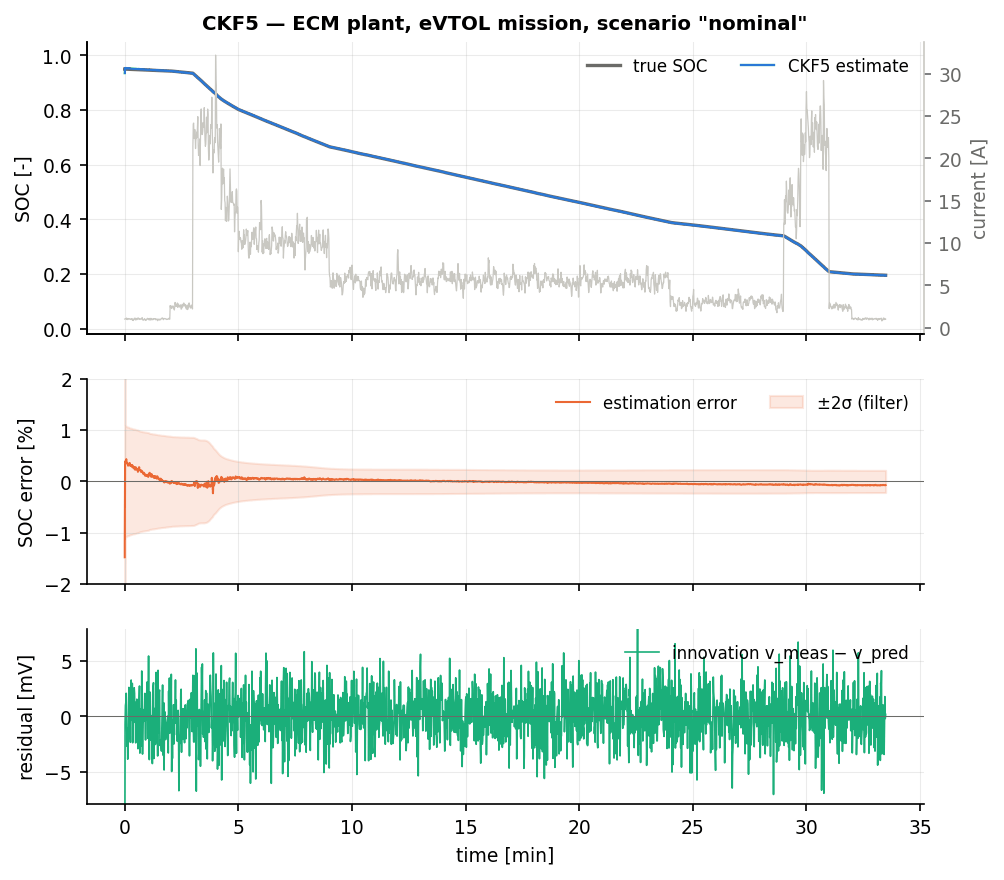
\includegraphics[width=\textwidth]{figures/cell_CKF5_nominal.png}
\caption{CKF5 on the nominal eVTOL mission: true and estimated SOC (top), estimation error with the $\pm 2\sigma$ band when available (middle), voltage residual (bottom).}
\end{figure}
\begin{figure}[H]\centering
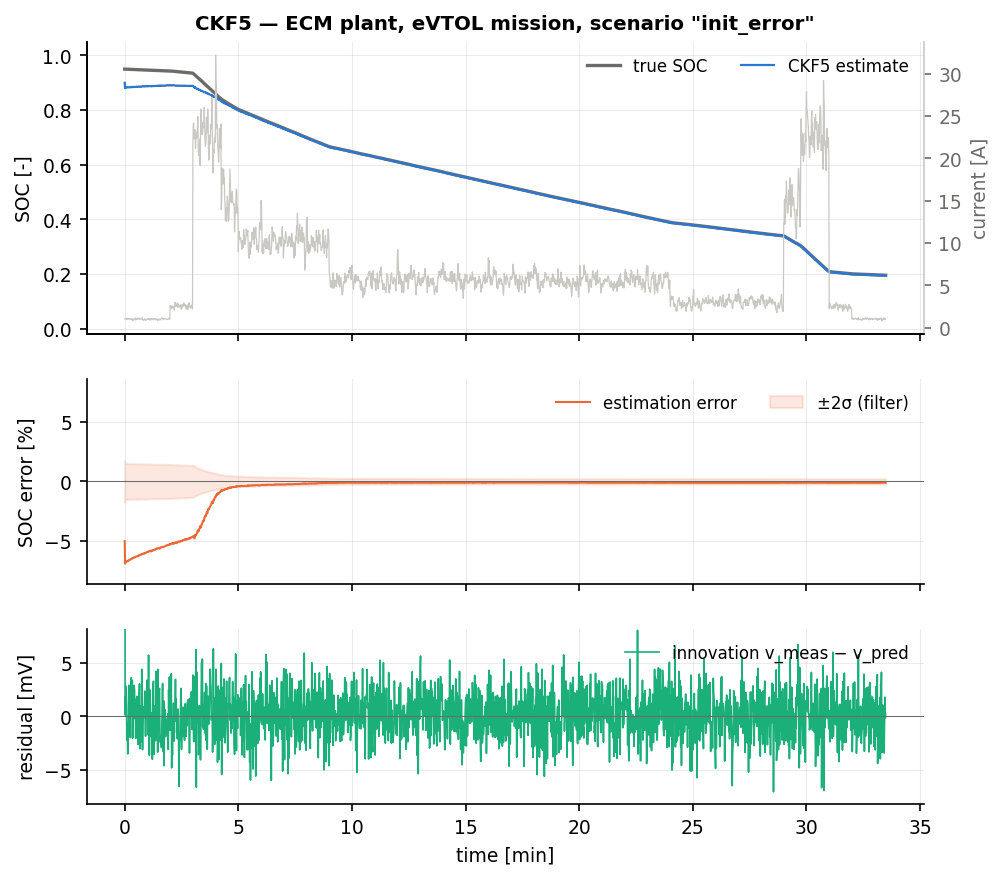
\includegraphics[width=\textwidth]{figures/cell_CKF5_init_error.png}
\caption{CKF5 with a 35\,\% initial SOC error.}
\end{figure}

All numbers are three-seed means in per cent SOC.

The most striking result is not in any single column but in the comparison across chapters:
\textbf{the CKF5, the DD2/CDKF (Chapter~\ref{ch:cdkf}) and the $3$-point Gauss--Hermite filter
(Chapter~\ref{ch:ghkf}) produce identical metrics to two decimals in all twelve ECM scenarios
and all nine SPM scenarios.} These are three independently derived rules --- a spherical-radial
cubature rule, a Stirling interpolation with step $h = \sqrt3$, and a tensor-product quadrature
--- that all integrate polynomials up to degree five exactly and all place their points at
$\sqrt3$ or $\sqrt{n_x+2}$ standard deviations. Their agreement is a strong mutual validation
of the three implementations and a concrete illustration of the ``numerical integration
perspective'' on Gaussian filters~\cite{wu2006numerical}: once the degree of exactness is
fixed, the specific rule matters far less than the degree.

Against the third-degree CKF the fifth-degree rule helps where the theory says it should ---
when the prior is wide. \texttt{aged\_cell}: $2.50/1.54\,\%$ against the CKF's $2.87/1.79\,\%$,
with the peak error falling from $9.6\,\%$ to $8.0\,\%$, which brings it level with the EKF
($1.18/1.52\,\%$). \texttt{outliers}: $0.31/0.08\,\%$, with $t_{\text{conv}} = 0$ against the
CKF's $4$\,s. Where the prior is tight the two are indistinguishable: \texttt{nominal}
$0.08/0.05\,\%$ for both, and \texttt{cold}, \texttt{hot}, \texttt{current\_bias},
\texttt{noise\_step} and \texttt{preisach} agree to within a hundredth of a per cent.

It is not uniformly better. \texttt{init\_error} is marginally worse ($1.85/0.12\,\%$,
$t_{\text{conv}} = 229$\,s, against $1.64/0.09\,\%$ and $221$\,s), because the higher-degree
rule reaches further ($\sqrt{n_x+2} = 2.45\sigma$ against $2\sigma$) into a region where the
OCV curve is not polynomial at all. \texttt{param\_mismatch} is worse ($1.84/1.79\,\%$ against
$1.56/1.59\,\%$) and \texttt{combined} is worse ($14.64/11.96\,\%$ against $13.07/11.26\,\%$);
both are model-error scenarios in which integrating the \emph{wrong} model more accurately is
no help --- a point worth keeping in mind whenever a higher-order filter is proposed as a cure
for a modelling problem. \texttt{sensor\_dropout} is a wash at $2.75/1.86\,\%$ against
$2.83/1.92\,\%$, both far behind the EKF's $0.72/0.46\,\%$.

\paragraph{SPM plant: structured model error.}
\begin{figure}[H]\centering
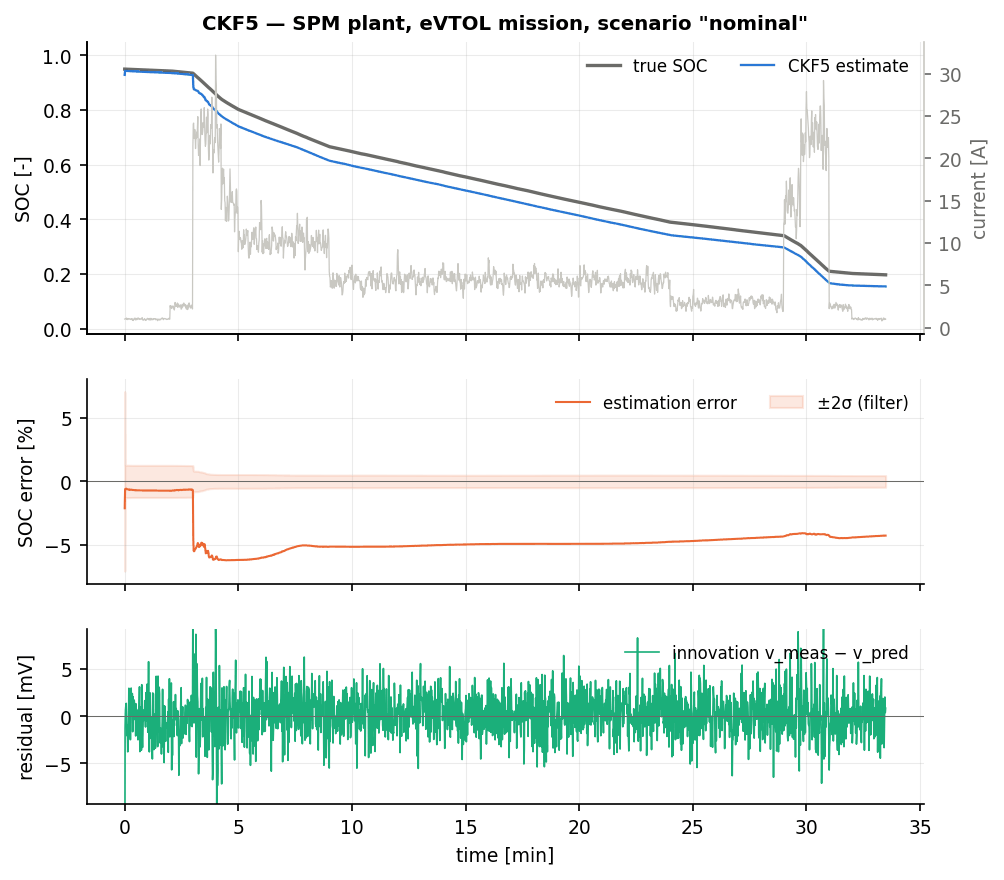
\includegraphics[width=\textwidth]{figures/cellspm_CKF5_nominal.png}
\caption{CKF5 on the nominal mission with the electrochemical (SPM) plant.}
\end{figure}
The SPM block of the table is a different kind of test. The plant is the electrochemical
single-particle model; the estimator still runs a 2-RC equivalent circuit, fitted to that plant,
which leaves a \emph{structured} residual of about $4$\,mV (Butler--Volmer kinetics and
solid-phase diffusion that no 2-RC circuit can reproduce) and a slow second branch,
$\tau_2 = 556$\,s. Over a $33$-minute mission a $556$\,s pole barely relaxes, so $v_2(t)$ is
close to an affine ramp --- and so is $\ocv(\soc(t))$ while the cell discharges at a roughly
constant rate. The two channels through which the measurement sees the state,
$(\partial\ocv/\partial\soc)\,\delta\soc$ and $-\delta v_2$, are therefore nearly collinear in
the information accumulated over the flight: the pair $(\soc, v_2)$ is close to unobservable,
and no filter can decide whether a persistent few-millivolt residual belongs to the slow RC
branch or to the state of charge. Because that direction is weakly observable, a $4$\,mV
structured error maps onto \emph{several per cent} of SOC instead of the
$4\,\text{mV}/0.8\,\text{V}\approx0.5\,\%$ a well-conditioned channel would give. This
$(\soc,v_2)$ ambiguity, not the size of the residual, is the mechanism behind the
$3.7$--$4.6\,\%$ band in which the whole classical family sits.

The fifth-degree rules sit at the bad end of the band: $4.61\,\%$ on SPM \texttt{nominal}
against the EKF's $3.73\,\%$ and the LKF's $1.72\,\%$, $8.74\,\%$ on \texttt{cold} against
$7.35\,\%$, $8.24\,\%$ on \texttt{sensor\_dropout} against $5.31\,\%$, $4.90\,\%$ on
\texttt{param\_mismatch} against $3.13\,\%$. They are statistically indistinguishable from the
third-degree CKF ($4.62$, $8.72$, $8.24$, $4.81\,\%$) --- the extra degree of exactness buys
nothing at all here --- and the ordering across the family is monotone in the point spread:
LKF (frozen tangent) $1.72$, EKF/IEKF (tangent at the mean) $3.66$--$3.73$, UKF
($0.2\sigma$ points) $3.96$, the degree-three and degree-five rules ($2\sigma$ and
$2.45\sigma$) $4.61$--$4.62$. The reason is the ambiguity above: a statistical linearisation
over a wide prior returns the \emph{chord} of the OCV curve, which is steeper than the tangent
over most of the mission, so these filters believe the OCV channel is more informative than it
is and commit harder to the direction that carries the structured error. The exception is
\texttt{outliers} ($2.27\,\%$), better than on the ECM plant for everyone because the corrupted
samples widen the effective innovation covariance. Nothing diverges; every SPM error is a bias,
not a drift ($t_{\text{conv}} = 0$ throughout).

\section{Summary}
The fifth-degree cubature filter is the right choice when the prior is genuinely wide and the
nonlinearity is smooth: on this benchmark it cuts the \texttt{aged\_cell} error by $15\,\%$ and
the \texttt{outliers} convergence time to zero relative to the third-degree rule at three times
the cost, and it matches it exactly when the prior is tight. It is not a remedy for model error
--- on \texttt{combined}, \texttt{param\_mismatch} and every SPM row it is equal to or slightly
worse than the cheaper rule --- and its $2n_x^2+1$ points and negative axial weight for
$n_x>4$ limit it to low-dimensional problems. For $n_x = 4$ it is a well-conditioned special
case: the axial weight is exactly zero and all remaining weights are positive. If fifth-degree
accuracy is what you want, take it from the DD2 filter of Chapter~\ref{ch:cdkf}, which delivers
the identical numbers at a third of the cost.
